\subsection{Build a Vocabulary of Audible Concepts}
\label{sec:vocab}

\begin{table}
\centering
\caption{Possible Audible Event Terms from Probase}
\label{tab:audible}
\small
\begin{tabular}{|l|l|} \hline
%\multicolumn{2}{|c|}{Probase} 	\\ \hline
{\bf Concepts} & {\bf Entities} \\ \hline \hline
sound & barking dog, music, {\em classical}\\ \hline
noise & siren, traffic, {\em light} \\ \hline
animal & dog, cat, snake	\\ \hline
sound effect & chorus, gunshot, {\em delay}\\ \hline
musical instrument & 	guitar, oboe, trumpet \\ \hline
%\multicolumn{2}{|c|}{WordNet} 	\\ \hline
%sound & voice, ring, unison	\\ \hline
%noise & clack, howl, thunder	\\ \hline
\end{tabular}
\end{table}

We create the audible concept vocabulary by a bootstrapping process.
Each iteration involves a ``growing phase'', which enlarges the 
current pool of audible concepts by including
additional terms from both an online sound search engine and a knowledge base,
and a ``filtering phase'', which removes some of the 
terms which are deemed inaudible from the current pool, 
using the same sound search engine.
The iterations stop when no new terms can be added after the filter phase. 
The final pool of concepts become the vocabulary of audible events.

The knowledge base we use for this purpose is called
Probase\cite{wu2012probase}, which is a probabilitic taxonomy of terms
organized in isA (or concept-entity) relations.
%\footnote{Hypernymy relation, also known as
%concept-entity relation, is the most 
%important relation in Probase, but there are other relations as well.}.
%and WordNet\cite{miller1995wordnet}. 
Each isA pair ($c$, $e$)
%\footnote{Here $c$ stands for a concept and
%$e$ stands for an entity and the two are related by isA relation: 
%$e$ isA $c$.} 
is associated with a frequency which is the
number of evidences that support this isA relation in a large text corpus, 
and two probability scores known as typicality, defined by
$P(e | c)$ and $P(c | e)$, which are calculated from the statistics of the
occurrences of terms $e$ and $c$ in the corpus.

We start the bootstrapping by creating an initial pool of
seed candidate event terms, which were the $k$ most typical
entities (by typicality $P(e | c)$)
under the concept terms such as ``sound'', ``noise'', ``musical instruments'',
etc.  \tabl{audible} gives the some examples of these candidate audible events 
terms discovered from Probase. One can see that not all of these terms
are truly audible events (those italicized terms in the table). 
We will remove such noises in the filtering phase.

In the {\bf growing phase}, we enrich the current pool by adding related terms
from two sources. We first query a sound search engine
\footnote{We use \url{http://www.freesound.org} and \url{http://www.findsounds.com} for this purpose.}
for each existing terms in the pool. The resulting clips for each query
(e.g., ``hunt dog'') carry tags such as ``labrador'' and ``puppy''. 
All such terms
which exist in Probase as entities (i.e., as $e$ in an isA pair) and
are not already in the current pool are considered new candidates.
We further expand the set of new candidates by clustering them 
under different super-concepts. During clustering, we represent each
new term as a vector if its super-concepts in Probase and compute distance
between any two by Cosine similarity. This way, we could group different 
variants of dogs together under the concept ``dog''. Since these variants
are probably audible, we deduce that other entities under ``dog'' are also
audible, and therefore add the most typical entities under ``dog'' which
are not in the pool as new candidate terms as well. \fig{expand} illustrate
this process.

\begin{figure}[th]
\centering
\epsfig{file=figures/expand.eps, width=0.8\columnwidth}
\caption{Expansion using Probase}
\label{fig:expand}
\end{figure}


In the {\bf filtering phase}, every new candidate term from this iteration
is searched in the sound search engine. We look at the information of the
returned audio clips for each term. All clips which are shorter than 0.1 seconds
or longer than 30 seconds are removed, because these are usually not a single
event by our experience. Finally we filter out terms which have
fewer than 10 resulting clips, and keep the rest in our pool and go on to
the next iteration. 


